\section{Designing the Board}
\label{sec:designing_playing_field}

As stated in \autoref{sec:requirements}, the game will be displayed as a 2D environment instead of 3D, since the focus of this project is not on realistic graphical presentation, but on the combination of engaging gameplay and education.
However, there are still different approaches when designing the playing field.
This section will focus on these approaches and argue why some solutions have been chosen over others.

\subsection{Free Environment vs. Tiles}
When approaching the design of a 2D environment, it might be possible to design the layout as being free or limited.
In a free environment, the cell would be able to stop at any point.
This approach is seen in the game Osmos, that is similar to our game without the programming aspect.
The player can move a cell freely in the 2D environment to eat smaller cells and each level has a specific objective.
However, the free environment approach would possibly increase the difficulty of programming the cell in contrast to a tile-based approach to design.
The reader might imagine, that it is more difficult to program a cell to move in all possible directions than in for example 4 or 6.
When saying tiles we refer to typical board games such as chess and checkers.\newline

Using tiles would limit the available movements of each cell into x number of directions, where x equals the amount of sides on a single tile..
The question is then whether the tile-based approach would limit the player too much, making the game less engaging and too easy.
However, a similar question can be applied to the free environment approach, whether a free environment would make it game stoo difficult and thereby scare some users away.\newline

We have chosen to design the playing field as a tile-based board game, since we do not think that the limitation of tiles makes the programming of the cells too easy.

\subsection{Designing the Tiles - Polygons}
Polygons are closed 2D objects, that have more than 2 sides.
The smallest polygon in term of sides is therefore the triangle.
Bizingo is a board game, that uses triangle tiles.
It is far more common to see games that use either square or hexagonal tiles.
Therefore, they both have the appeal of being more recognizable to the user, making the game easier to learn.
We will mainly discuss the pros and cons with square and hexagonal tiles.

\subsubsection{Squares vs Hexagonal tiles}
In terms of the players ability to move, square tiles would allow for 4 directions of movement (8 if diagonal movement is allowed), while hexagonal tiles would allow for 6.
Hexagonal tiles when placed in a board will never have an adjacent tile that is not locate along an edge.\newline

Some may argue, that if 6 sided tiles are more realistic than 4 sided, then why not go further and use 8 or 10 sided tiles.
However 8 or 10 sided tiles cannot be packed tightly, creating holes in the board, illustrated on \autoref{fig:tiles_dif}.

\begin{figure}[h]
  \centering
    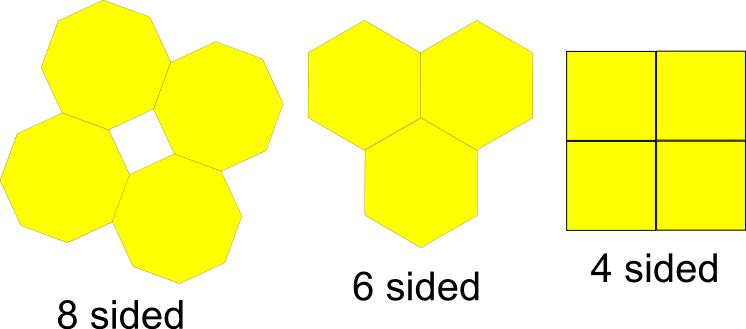
\includegraphics[width=0.6\textwidth]{img/8-6-4-sided-tiles.png}
  \caption{Difference between 8, 6, and 4 sided tiles}
  \label{fig:tiles_dif}
\end{figure}

In the end, it came down to a design decision on the group's behalf between square and hexagon tiles.
The hexagon approach would allow for tight packing of the tiles on the board and a larger range of motion with all adjacent tiles being located along edges, which is what the group desired.



